\documentclass[a4paper,12pt]{article}
\usepackage{fontspec} % This is to set system fonts like Arial
\usepackage[utf8]{inputenc}
\usepackage{array}
\usepackage{geometry}
\usepackage{tabularx}
\usepackage{graphicx}
\usepackage{enumitem}
\usepackage{longtable}
\usepackage{xcolor}
\usepackage[hidelinks]{hyperref}
\usepackage{titlesec} % For section formatting
\usepackage{tocloft}  % For TOC customization

% Set Arial font
\setmainfont{Arial}

% Numbering up to sub-subsections
\setcounter{secnumdepth}{3} % Include sub-subsections in numbering
\setcounter{tocdepth}{3}    % Include sub-subsections in TOC

% Customizing bullet points
\setlist[itemize,1]{label=•} % First-level bullets
\setlist[itemize,2]{label=◦} % Second-level bullets
\setlist[itemize,3]{label=–} % Third-level bullets

% Page setup
\geometry{top=2.5cm, bottom=2.5cm, left=2.5cm, right=2.5cm}

% Section heading formatting (if you need more control over boldness)
\titleformat{\section}[block]{\normalfont\Large\bfseries}{\thesection}{1em}{}
\titleformat{\subsection}[block]{\normalfont\large\bfseries}{\thesubsection}{1em}{}
\titleformat{\subsubsection}[block]{\normalfont\normalsize\bfseries}{\thesubsubsection}{1em}{}

\setlength{\cftbeforesecskip}{10pt} % Space before section entries
\setlength{\cftbeforesubsecskip}{8pt} % Space before subsection entries
\setlength{\cftbeforesubsubsecskip}{6pt} % Space before sub-subsection entries

\begin{document}

% Horizontal line
\noindent\rule{\textwidth}{1pt}

\vspace{1cm}

% Title
\begin{flushright}
    \Huge\textbf{Software Requirements} \\[0cm]
    \Huge\textbf{Specification} \\[0.5cm]
    \Large\textbf{for} \\[0.5cm]
    \Huge\textbf{Automated Lecture Hall Booking Portal} \\[1cm]
    \Large\textbf{Version 0.1}
\end{flushright}

\vspace{1cm}

% Prepared by section
\begin{flushright}
    \Large\textbf{Prepared by-}
\end{flushright}

\vspace{0.5cm}

% Group 12 and Group Name (aligned)
\begin{tabular}{@{}p{0.45\textwidth}p{0.45\textwidth}@{}}
    \textbf{Group 12} & \hfill\textbf{Group Name: Aviators} \\
\end{tabular}

\vspace{0.5cm}

\begin{flushright}
\begin{tabular}{@{}p{0.05\textwidth} p{0.3\textwidth} p{0.15\textwidth} p{0.5\textwidth}@{}}
    \textbf{\#} & \textbf{Name} & \textbf{Roll No.} & \textbf{Email} \\[0.5cm] % Adds vertical space after the header row
    • & Chaitanya Bramhapurikar & 230305 & \href{mailto:bcvishwas23@iitk.ac.in}{bcvishwas23@iitk.ac.in} \\
    • & Rahul Meena & 230832 & \href{mailto:rahulkcm23@iitk.ac.in}{rahulkcm23@iitk.ac.in} \\
    • & Bhavya Chauhan & 230294 & \href{mailto:bhavyach23@iitk.ac.in}{bhavyach23@iitk.ac.in} \\
    • & Atharv Phirke & 230238 & \href{mailto:atharvp23@iitk.ac.in}{atharvp23@iitk.ac.in} \\
    • & Aaradhya Rohi & 230011 & \href{mailto:aaradhya23@iitk.ac.in}{aaradhya23@iitk.ac.in} \\
    • & Chaudhari Divyesh & 230325 & \href{mailto:divyesh23@iitk.ac.in}{divyesh23@iitk.ac.in} \\
    • & Devansh A Dhok & 230354 & \href{mailto:devanshad23@iitk.ac.in}{devanshad23@iitk.ac.in} \\
    • & Areen Mahich & 230188 & \href{mailto:areenm23@iitk.ac.in}{areenm23@iitk.ac.in} \\
    • & Daksh Dua & 220321 & \href{mailto:dakshdua22@iitk.ac.in}{dakshdua22@iitk.ac.in} \\
    • & Avantika Rohite & 230245 & \href{mailto:avantikar23@iitk.ac.in}{avantikar23@iitk.ac.in} \\
\end{tabular}
\end{flushright}



\vspace{1cm}

% Course and Mentor TA
\begin{flushright}
\begin{tabular}{rl}
    \textbf{Course:} & CS253 \\
    \textbf{Mentor TA:} & Souvik Banerjee\\
    \textbf{Date:} & 24 January 2025
\end{tabular}
\end{flushright}

\newpage

% Table of Contents
\tableofcontents
\newpage

% Revisions Section
\section*{Revisions}
\begin{tabular}{|l|l|l|l|}
\hline
\textbf{Version} & \textbf{Primary Author(s)} & \textbf{Description of Version} & \textbf{Date Completed} \\
\hline
0.1 & Group 12 & Initial Draft & 24/01/25 \\
\hline
\end{tabular}
\newpage

% Introduction
\section{Introduction} \label{sec:intro}
\subsection{Product Scope} \label{subsec:product_scope}
Our product, an \textbf{``Automated Lecture Hall Booking Portal''} is designed to streamline and simplify the process of booking lecture halls for various purposes in IIT Kanpur. It allows faculties, administrators and other authorized personnel to efficiently manage Lecture Hall bookings. This system drastically reduces manual efforts in lecture hall bookings, also addressing issues such as manual error, double bookings and scheduling conflicts. Users can view real-time availability of a lecture hall for all the time slots, request bookings and receive quick confirmation.
The system provides integration with institutional calendars enabling seamless coordination of lectures, events etc. Scope extends to features such as role-based access, user authentication and advanced search options for filtering lecture halls based on capacity, equipment and other features.


\subsection{Intended Audience and Document Overview} \label{subsec:intended_audience}
This document is intended for \textbf{developers}, \textbf{professors} and \textbf{TAs} evaluating the same for the course project, and \textbf{end-users}, with the last category of audience likely to be one of the below-mentioned categories:

\begin{itemize}
    \item \textbf{Professors:}  Professors can use this portal for booking lecture halls for their course lectures and labs(for the entire semester), Quizzes, Make up classes and talks from researchers and other professors of the same or other universities to showcase their research work.
    \item \textbf{Clubs/Societies/Fests:} Heads of clubs, societies, fests and cells may also use this portal to book lecture halls for their events for the campus community.
    \item \textbf{Lecture Hall Administration:} They shall be the ones coordinating between the institute bodies(DoAA/DoSA) and the above two mentioned here, and cancel/approve booking requests based on availability. 

\end{itemize}
Developers, professors and TAs should have a look at the sections \ref{sec:description}, \ref{sec:specific_reqs} and \ref{sec:nonfunctional} of the document in order to have a strong understanding of the technical aspects of the portal, along with the functionality.
On the other hand, end-users as elaborated above, just need to go through sections \ref{subsec:overview} and \ref{subsec:functionality}, just to understand the functioning of the overall software.
Everyone reading this document must refer to \ref{subsec:definitions} and the Appendix in case they encounter terms unfamiliar to them. 
\newpage
\subsection{Definitions, Acronyms, and Abbreviations \label{subsec:definitions}}

% /////////////////////////////////


\renewcommand{\arraystretch}{1.8}
% Longtable with increased width
\begin{longtable}{|m{4cm}|m{12cm}|}
\hline
\textbf{Acronym} & \textbf{Description} \\
\hline
\endfirsthead
\hline
\multicolumn{2}{|c|}{\textbf{Definitions, Acronyms, and Abbreviations (cont.)}} \\
\hline
\textbf{Term} & \textbf{Description} \\
\hline
\endhead
\hline
\endfoot
\hline
\endlastfoot
ACID & Atomicity, Consistency, Isolation, and Durability \\ \hline
API & Application Programming Interface \\ \hline
AWS & Amazon Web Services \\ \hline
CSV & Comma Separated Values \\ \hline
DB & DataBase \\ \hline
DBMS & DataBase Management System \\ \hline
HTTPS & HyperText Transfer Protocol Secure \\ \hline
IT & Information Technology \\ \hline
JS & JavaScript \\ \hline
LHC & Lecture Hall Complex \\ \hline
MongoDB & Humongous DataBase \\ \hline
PDF & Portable Document Format \\ \hline
REST & Representational State Transfer \\ \hline
SMTP & Simple Mail Transfer Protocol \\ \hline
SQL & Structured Query Language \\ \hline
\end{longtable}


% Standard table with increased width
\begin{table}[h!]
\centering
\renewcommand{\arraystretch}{1.8}
\begin{tabular}{|m{4cm}|m{12cm}|} % Increased column widths
\hline
\textbf{Term} & \textbf{Definition} \\ \hline 
\textbf{Admin} & \parbox[t]{11cm}{Administrative. The term ‘admin’ refers to the IIT-K Lecture Hall Complex Office staff. This type of user has full control over the system’s operation.}
\\ \hline
\textbf{User} & \parbox[t]{11cm}{The term ‘User’ refers to the various entities/organizations in the IIT-K campus that need to request a Lecture Hall booking. Examples include Professors, Clubs, Student Placement Office.}
\\ \hline
\textbf{Web-app} & \parbox[t]{11cm}{A software application that runs on a web browser and can be accessed from any device with an internet connection.} 
\\ \hline
\end{tabular}

\label{tab:definitions}
\end{table}

\subsection{Document Conventions} \label{subsec:conventions}

The document adheres to the following font specifications to maintain consistency and readability:

\begin{enumerate}
    \item \textbf{Base Font:}
    \begin{itemize}
        \item The default font for the document is \textbf{Arial} with a base font size of \textbf{12pt}.
    \end{itemize}

    \item \textbf{Title Font Sizes:}
    \begin{itemize}
        \item \textbf{Document Title:} Set in \texttt{\textbackslash Huge}, approximately \textbf{24.88pt}.
        \item \textbf{Subtitles (e.g., "for," "Version 0.0"):} Set in \texttt{\textbackslash Large}, approximately \textbf{14.4pt}.
    \end{itemize}

    \item \textbf{Section Titles:}
    \begin{itemize}
        \item \textbf{Section Titles:} Set in \textbf{16.59pt}.
        \item \textbf{Subsection Titles:} Set in \textbf{14.4pt}.
        \item \textbf{Sub-subsection Titles:} Set in \textbf{12pt}.
    \end{itemize}

    \item \textbf{Other Text Elements:}
    \begin{itemize}
        \item \textbf{Prepared By:} The "Prepared By" label is set in \texttt{\textbackslash Large}, approximately \textbf{14.4pt}.
        \item \textbf{Tables and Lists:} All text within tables and lists is set to the base font size of \textbf{12pt}.
    \end{itemize}

    \item \textbf{Table of Contents:}
    \begin{itemize}
        \item The Table of Contents title and entries use the base font size of \textbf{12pt}.
    \end{itemize}

    \item \textbf{Revisions Table:}
    \begin{itemize}
        \item All text within the Revisions table is set to the base font size of \textbf{12pt}.
    \end{itemize}
\end{enumerate}

These font settings are designed to ensure a professional and cohesive appearance throughout the document.

\subsection{References and Acknowledgments} \label{subsec:refs}
\begin{itemize}
    \item IEEE Std 830-1998 IEEE Recommended Practice for Software Requirements Specifications. IEEE Computer Society, 1998.

\end{itemize}
We’d also like to acknowledge the help of our TA, \textbf{Mr. Souvik Mukherjee}, for their valuable input in the creation of this document. We also would like to thank \textbf{\href{https://www.cse.iitk.ac.in/users/isaha/}{Prof. Indranil Saha}} for teaching us the concepts of the course and guiding us.

\newpage

% Overall Description
\section{Overall Description} \label{sec:description}
\subsection{Product Overview} \label{subsec:overview}
The Automated Lecture Hall Booking Portal is a new, self-contained system designed to manage the scheduling and booking of lecture halls at IIT Kanpur. It is not a replacement for any existing system but an enhancement to current manual processes. The portal digitises the scheduling process and centralizes the user authentication system for secure role-based access. Users such as faculty, administrators, and other authorized personnel interact with the system to view lecture hall availability, book halls, and resolve scheduling conflicts. The system ensures efficient resource utilization by minimizing manual errors and efforts.

% Insert Flow diagram here
\begin{figure}[h] % 'h' places the figure approximately here
    \centering
    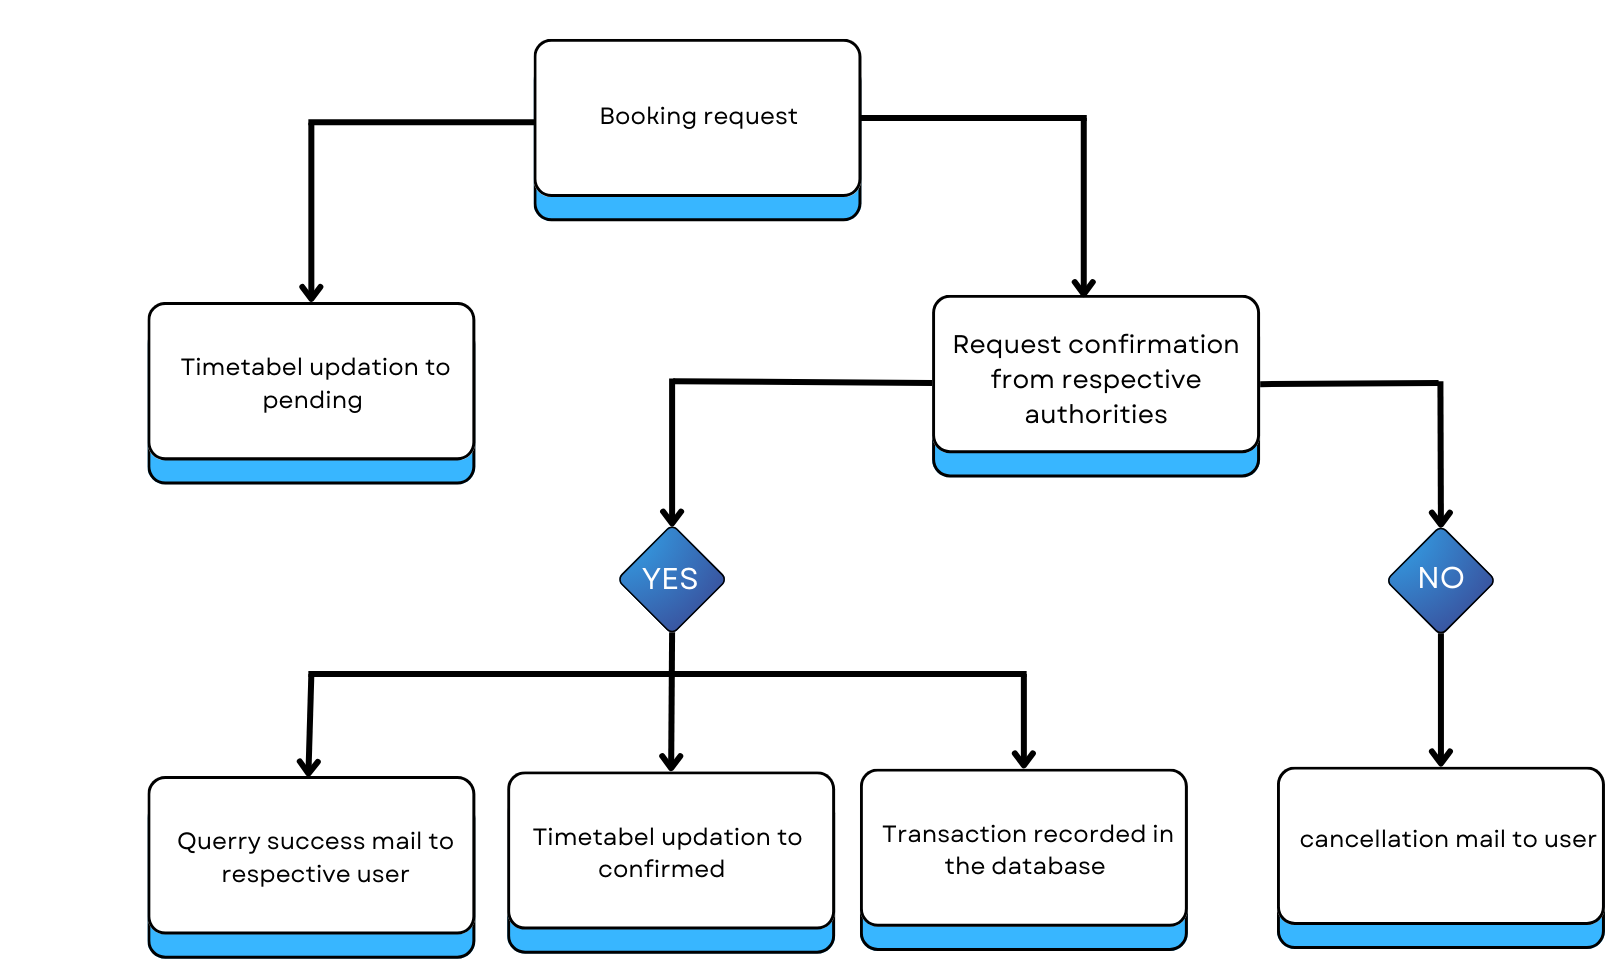
\includegraphics[width=\textwidth]{flow2.png} % Adjust the width as needed
    \caption{Flow Diagram}
    \label{fig:Flow Diagram} % Optional label for referencing
\end{figure}

\clearpage
\subsection{Product Functionality} \label{subsec:functionality}


\begin{figure}[h] % 'h' places the figure approximately here
    \centering
    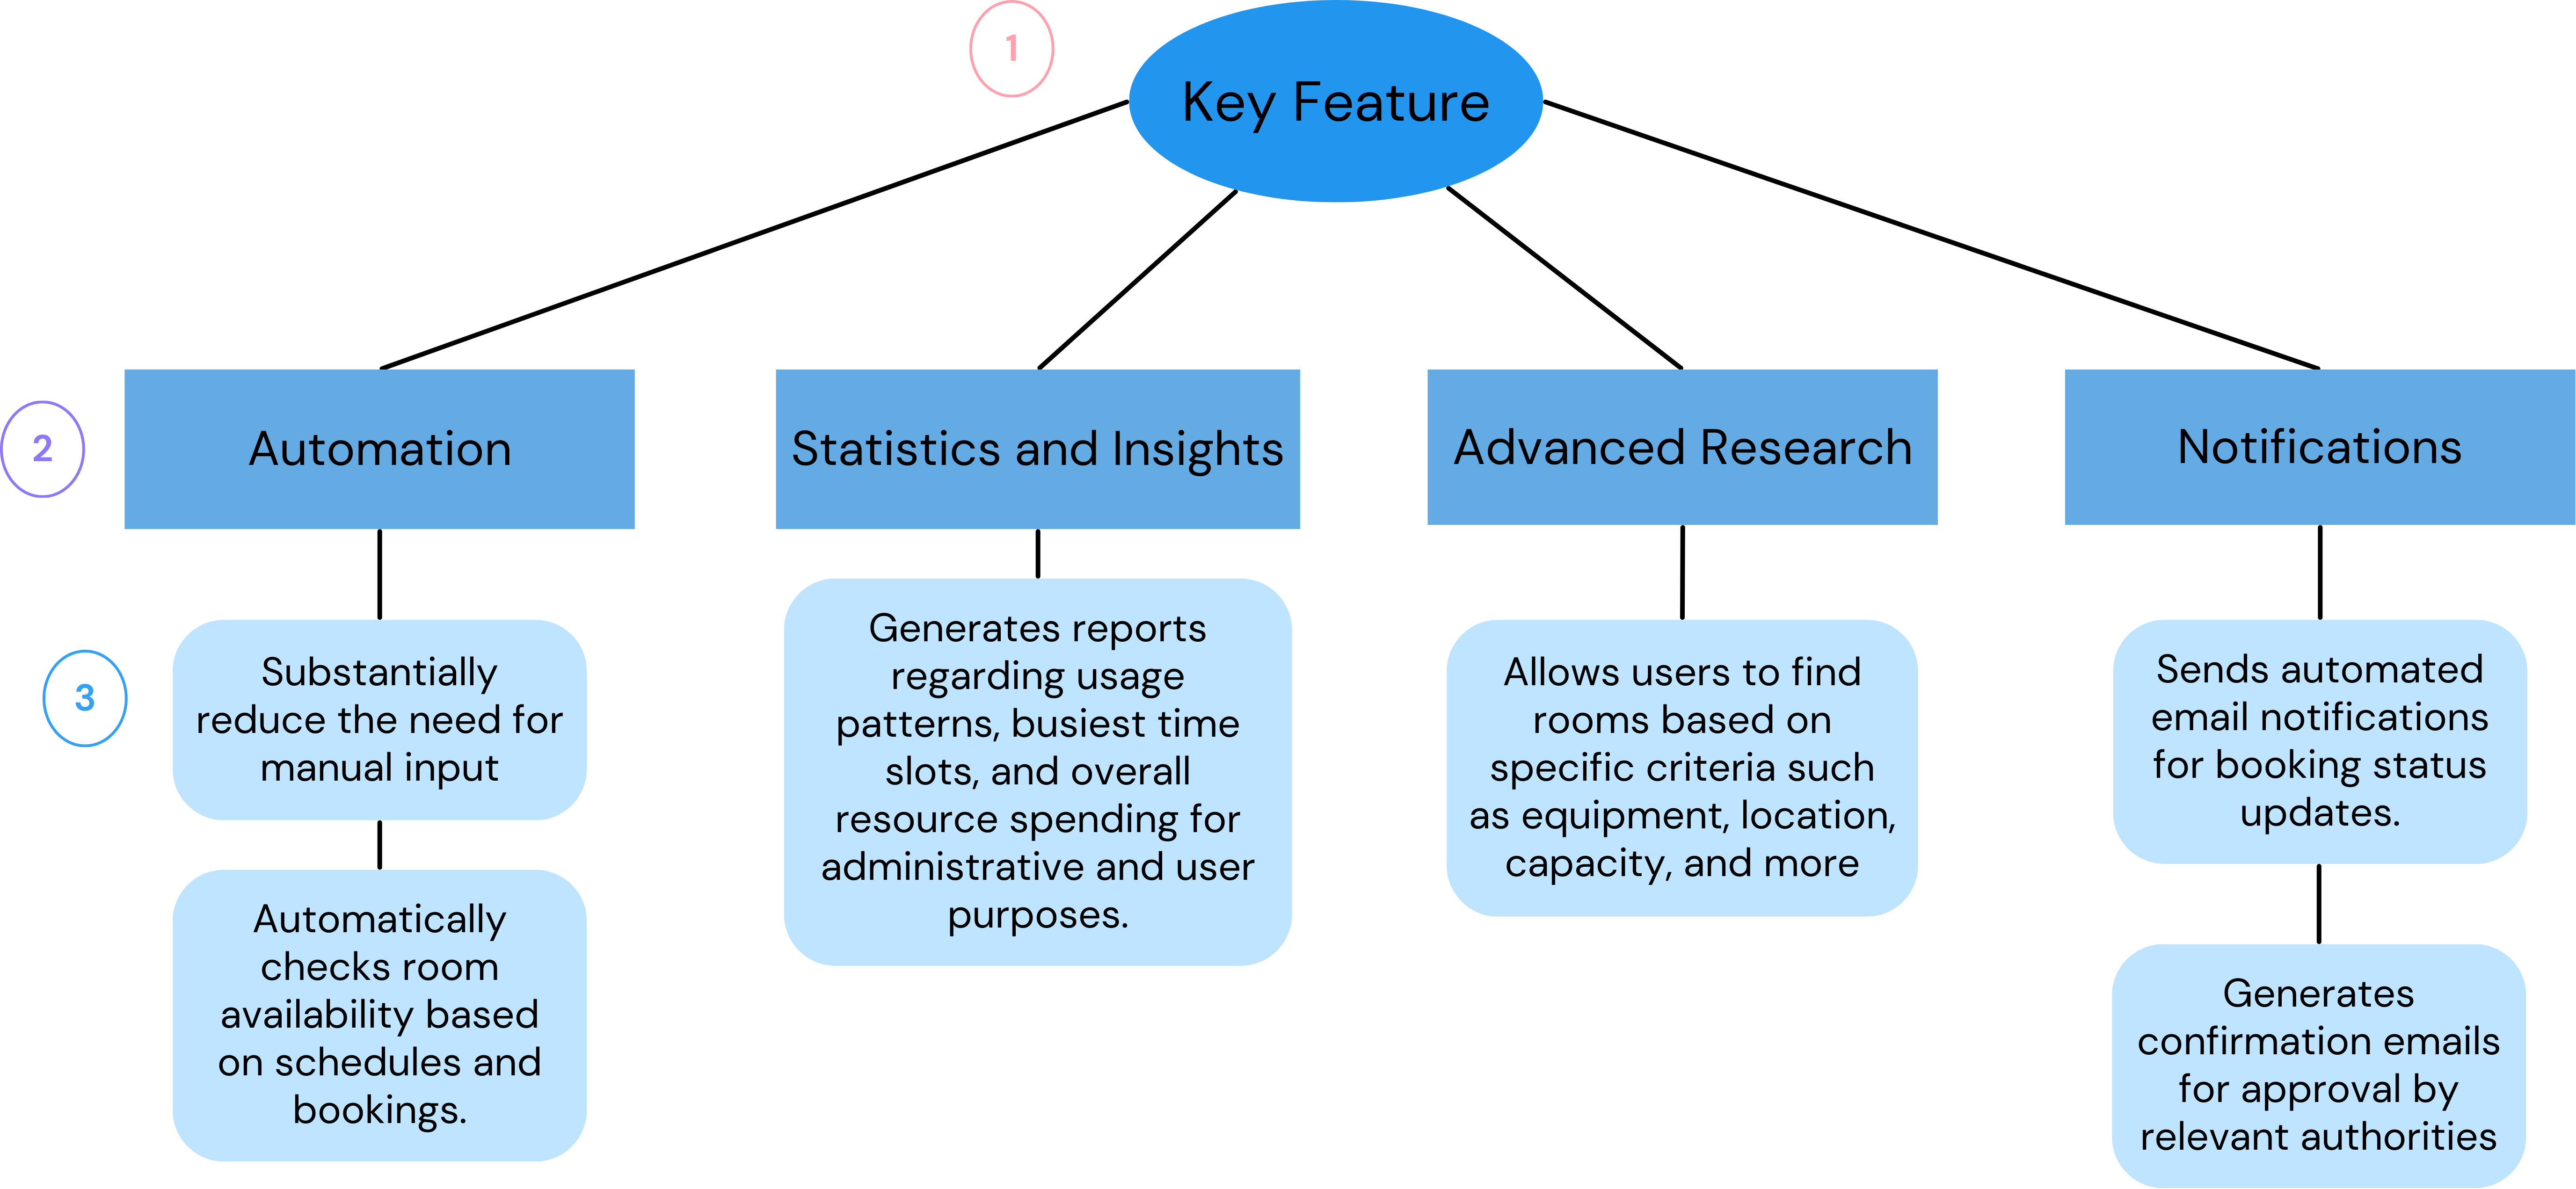
\includegraphics[width=\textwidth]{Key Feature (1).png} % Adjust the width as needed
    \caption{Product Features}
    \label{fig:Product Features} % Optional label for referencing
\end{figure}

\subsection{Design and Implementation Constraints} \\\label{subsec:constraints}
\begin{itemize}
    \item \textbf{Email Notification Service:}
    \begin{itemize}
        \item The system depends on IITK webmail or another SMTP service for sending notifications. Any service downtime, misconfiguration, or traffic surge could lead to communication issues. Retry mechanisms and error logging should be implemented to handle failures effectively.
        \item Scalability is required to handle high-traffic periods, such as during Semester Examination periods
    \end{itemize}
    \item \textbf{Integration with Institute’s academic Calendar:}
    \begin{itemize}
        \item The portal might need to sync with the institute’s academic calendar to avoid scheduling conflicts with pre-planned events and to prevent bookings on institute holidays.
    \end{itemize}
    \item \textbf{Performance and Resource Management:}
    \begin{itemize}
        \item Large report generation requires careful resource optimization to avoid overloading server CPU, RAM, and storage.
        \item The system should ensure minimal delays while processing or querying data for reports, even under high server loads.
    \end{itemize}
    \item \textbf{Browser and Device Compatibility:}
    \begin{itemize}
        \item The application must be compatible with modern web browsers (e.g., Chrome, Firefox, Edge). Features like JavaScript and cookies are essential for functionality, and support for outdated browsers will not be provided.
        \item The design should also ensure \textbf{responsiveness} for different screen sizes, including desktops, tablets, and smartphones, if required.
    \end{itemize}
    \item \textbf{Data Security and Integrity:}
    \begin{itemize}
        \item User data and reports must be protected against unauthorized access. Encryption should be used for sensitive data in transit and at rest.
        \item The system must adhere to IIT Kanpur’s IT security and data handling policies. Sensitive information like passwords and financial records must be stored securely using encryption.
    \end{itemize}
    \item \textbf{No Sign-Up Feature:}
    \begin{itemize}
        \item There will be no user self-registration; credentials must be created and distributed manually by the LHC Office Staff(admin).
    \end{itemize}
    \item \textbf{Interface Design:}
    \begin{itemize}
        \item The system must provide two separate interfaces: one for end-users (professors and club coordinators) and another for administrators (LHC office staff).
The interface should be accessible and responsive on both desktop and mobile devices.
    \end{itemize}
    \item \textbf{Hardware Dependency:}
    \begin{itemize}
        \item The system should integrate seamlessly with the LHC office's existing hardware and software systems.
    \end{itemize}
\end{itemize}

\newpage

\subsection{Assumptions and Dependencies} \\\label{subsec:assump_and_dependencies}
\subsubsection{Assumptions}
    \begin{itemize}
        \item \textbf{Database Availability:} The relational database (e.g., MySQL, PostgreSQL) will remain operational with minimal downtime and will scale to handle data growth as the system expands.
        \item \textbf{Authentication Systems:} Institutional authentication systems will function reliably to verify user roles (e.g., office staff, authorities) without errors or delays.
        \item \textbf{Email Services:} IITK webmail or another configured SMTP service will handle notification requests efficiently, even during periods of high traffic. Configuration changes will be minimal and well-documented.
        \item \textbf{Valid Input Data:} Users will input data in the correct format, reducing validation errors during report generation and ensuring smooth operation.
        \item \textbf{Network Stability:} The system assumes stable and reliable network connectivity to facilitate interactions between the database, SMTP service, and user interface components.
    \end{itemize}
\subsubsection{Dependencies}
    \begin{itemize}
        \item \textbf{Database Technology:} The system relies on a well-configured and operational database (MySQL, PostgreSQL) to store and retrieve data efficiently. Any downtime or misconfiguration could disrupt report generation and data consistency.
        \item \textbf{SMTP and Webmail Services:} The SMTP service, including IITK webmail, is critical for sending notifications. Failures, misconfigurations, or changes in these services could disrupt communication.
        \item \textbf{Authentication System:} Integration with institutional authentication systems is a core dependency. Changes in authentication protocols or system failures can block access for legitimate users.
        \item \textbf{Error Logging and Monitoring:} Dependencies exist on logging mechanisms to track and resolve database connection issues, SMTP failures, and report generation errors promptly. These logs should be easily accessible to administrators.
        \item \textbf{Server Resources:} Sufficient server resources (CPU, RAM, storage) must be available to support simultaneous requests for report generation, data queries, and notifications without performance degradation.
        \item \textbf{Network Connectivity:} Stable and fast network connectivity is required for real-time interactions between system components and to maintain uptime.
    \end{itemize}
\newpage
% Specific Requirements
\section{Specific Requirements} \label{sec:specific_reqs}
\subsection{External Interface Requirements}\label{subsec:ext_interface_reqs}
\subsubsection{User Interfaces}
The software application will provide intuitive and responsive interfaces accessible via web browsers and mobile devices. The User and Admin will have different roles while also sharing some elements of the functionalities and interface. Below are the graphical views of the User and Admin interfaces.

\begin{enumerate} [label=\Roman*.]
    \item \textbf{Login Screen:} 
    \begin{figure}[h!]
    \centering
    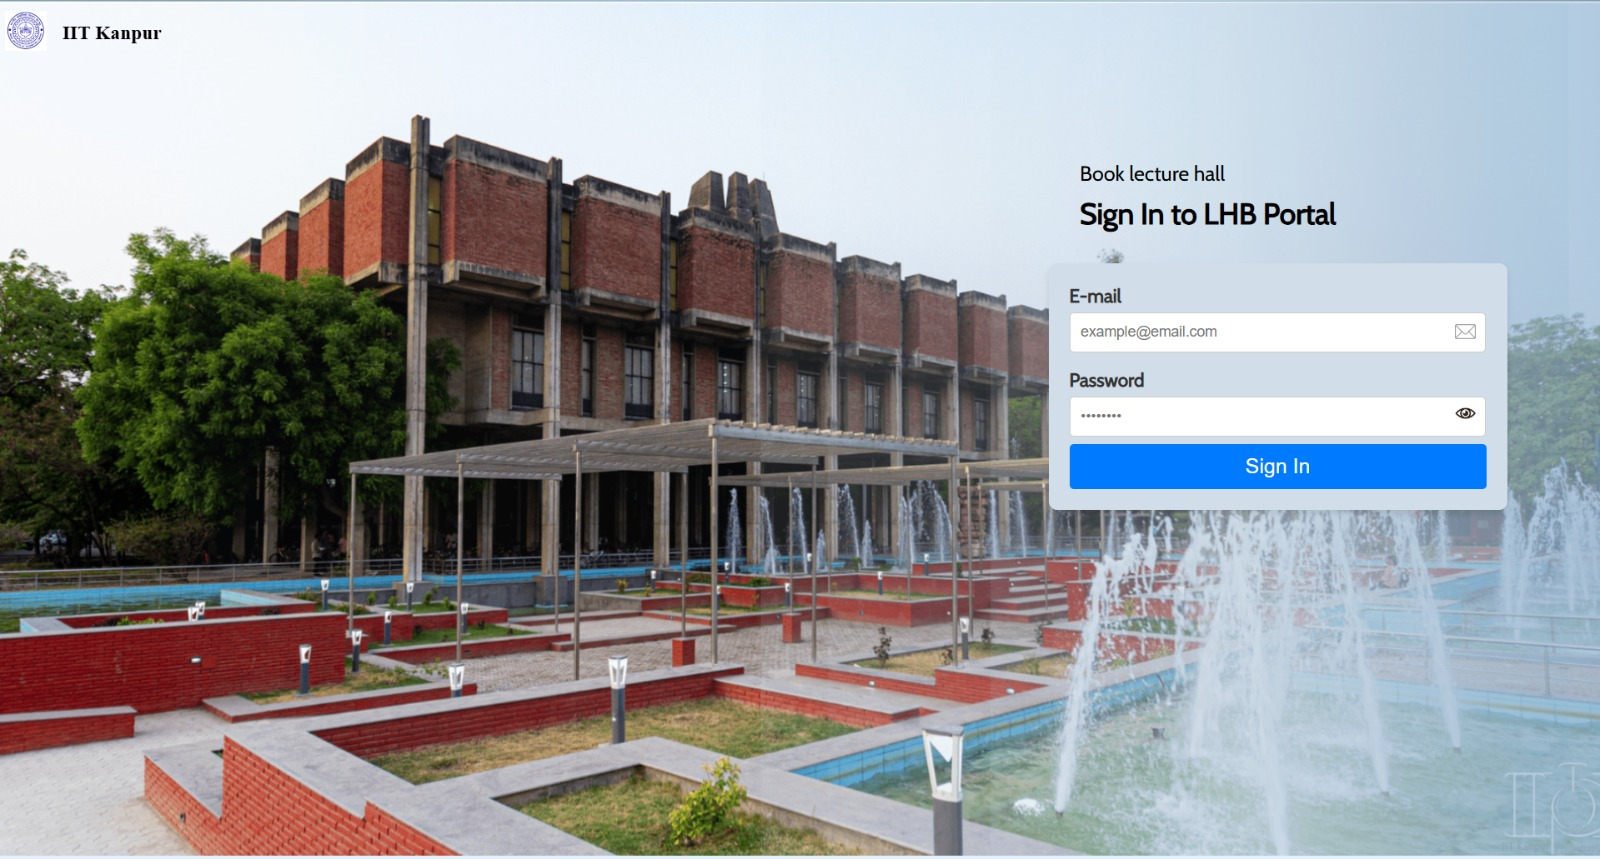
\includegraphics[width=1\textwidth]{login.jpg} 
    \caption{Login Screen}
    \label{Fig 3.1.1 : Login Screen}
\end{figure}
    \begin{itemize}
        \item \textbf{Description:}
        \begin{itemize}
            \item The login screen will allow users and admin to authenticate securely.
            \item Users and admin will enter their username and password.
            \item Buttons for “Sign In” will be provided.
            \item Validation messages will be displayed for incorrect credentials.
        \end{itemize}
        \item \textbf{Interaction:}
        \begin{itemize}
            \item Text fields for input.
            \item “Sign In” button to process login.
        \end{itemize}
    \end{itemize}
    \clearpage
   
    \item \textbf{Dashboard:}
     \begin{figure}[h!]
    \centering
    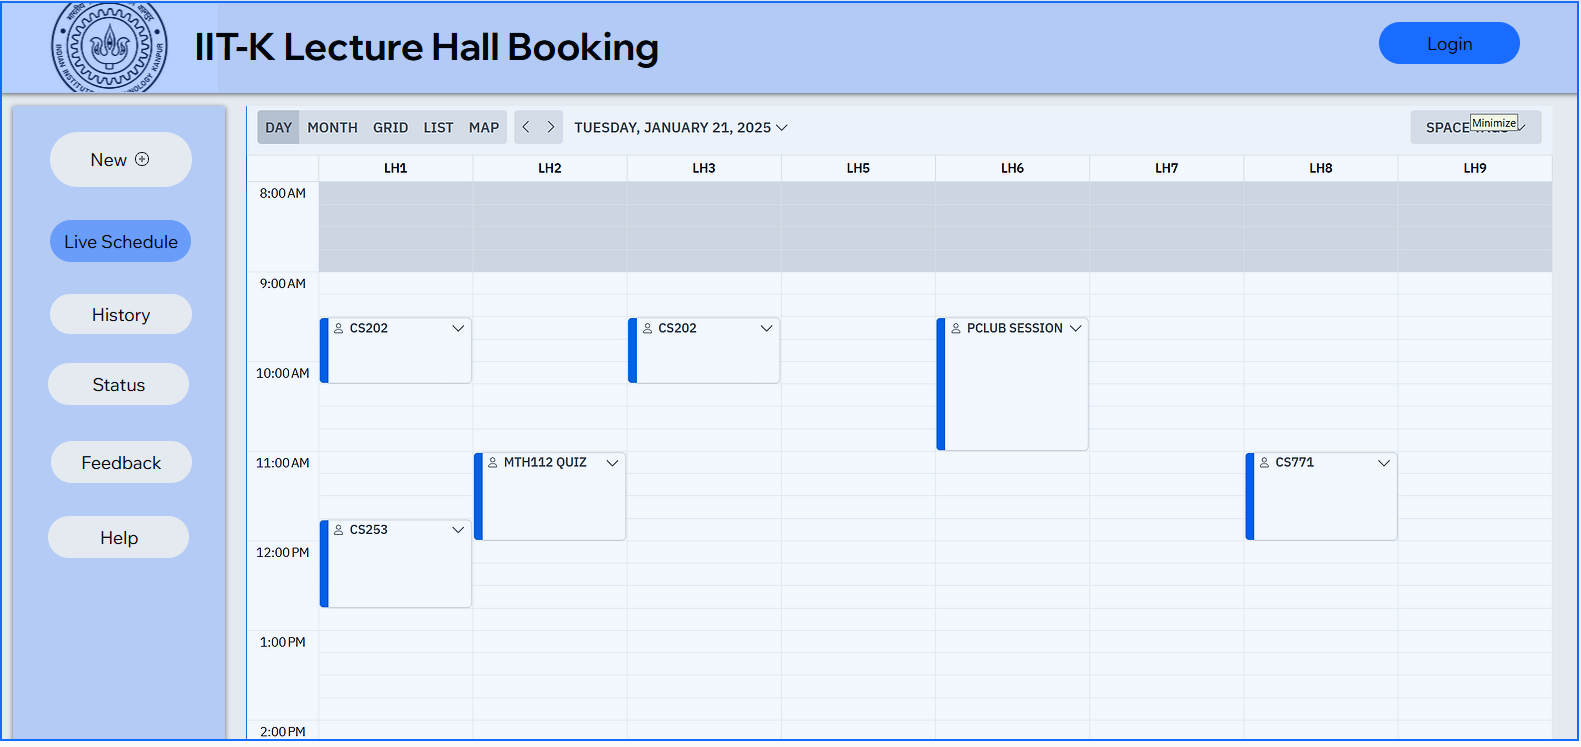
\includegraphics[width=1\textwidth]{time.png} 
    \caption{Dashboard}
    \label{dashboard}
    \end{figure}
    
    \begin{itemize}
        \item \textbf{Description:}
        The dashboard serves as the central hub for user interactions based on their roles.
The Live Schedule is the common element between both the User and Admin interface.
        
        \begin{itemize}
            \item User Role: Options to submit a new request, view the status of previous requests, and access notifications, provide feedback.
            \item Admin Role: Options to approve/reject requests, delete and view/search verification history.
        \end{itemize}
        \item Interaction:
        \begin{itemize}

            \item Live Schedule
            \item Drop-down menus, clickable cards, and quick navigation buttons.
            \item Notifications area for updates.
        \end{itemize}    
    \end{itemize}

    \clearpage
    
  
    \item \textbf{History Tab - User:} 
      \begin{figure}[h!]
    \centering
    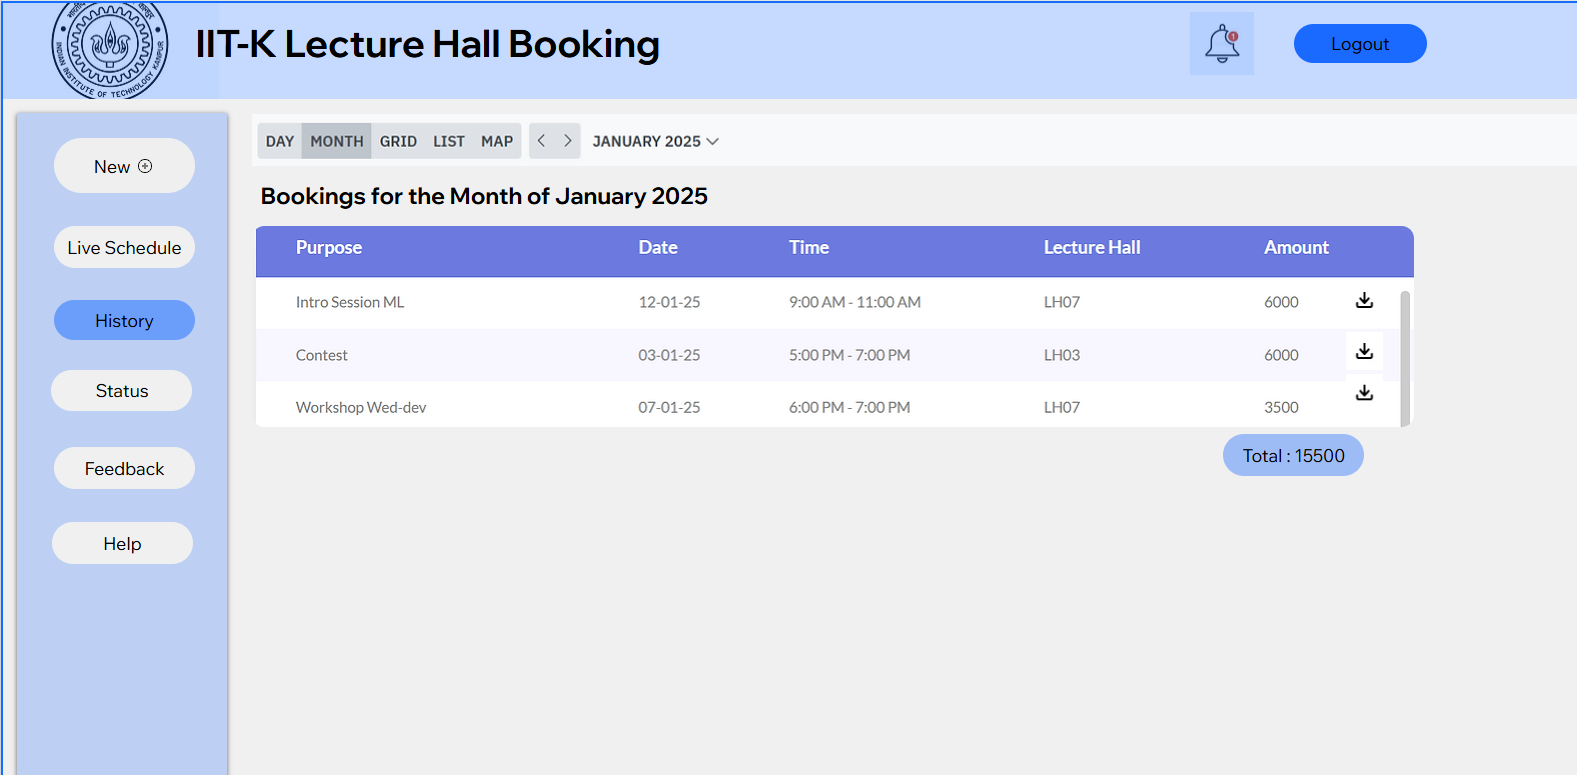
\includegraphics[width=1\textwidth]{his user.png} 
    \caption{User History}
    \label{history}
\end{figure}
    
    
    \begin{itemize}
        \item \textbf{Description:}
        \begin{itemize}
            \item The History Tab allows users to view their past bookings. 
            \item The Auto-Generated Bills can be downloaded from here.
            \item A table view displaying booking details such as: Purpose, Date, Time, Lecture Hall number and Amount.
        \end{itemize}
        \item \textbf{Interaction:}
        \begin{itemize}
            \item A search bar to filter bookings by date or month.
            \item Dropdown filters for easy navigation.
            \item An option to download bills for individual bookings.
        \end{itemize}
    \end{itemize}
\clearpage

% \begin{figure}[h!]
%     \centering
%     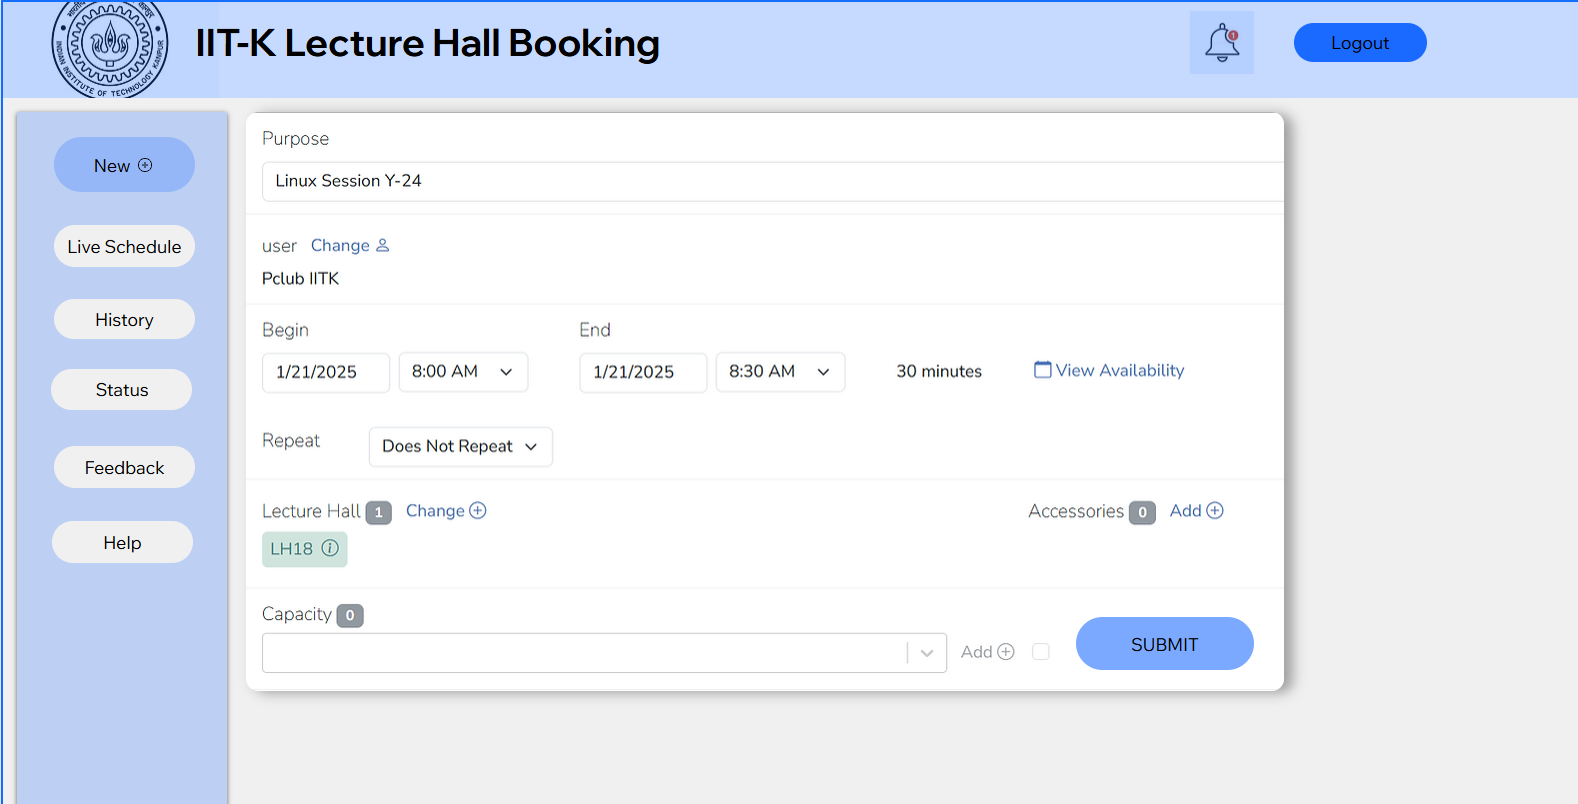
\includegraphics[width=1\textwidth]{form.png} 
%     \caption{Request Submission Form}
%     \label{form}
% \end{figure}
    
    \item \textbf{Request Submission Form:}
    \begin{figure}[h!]
    \centering
    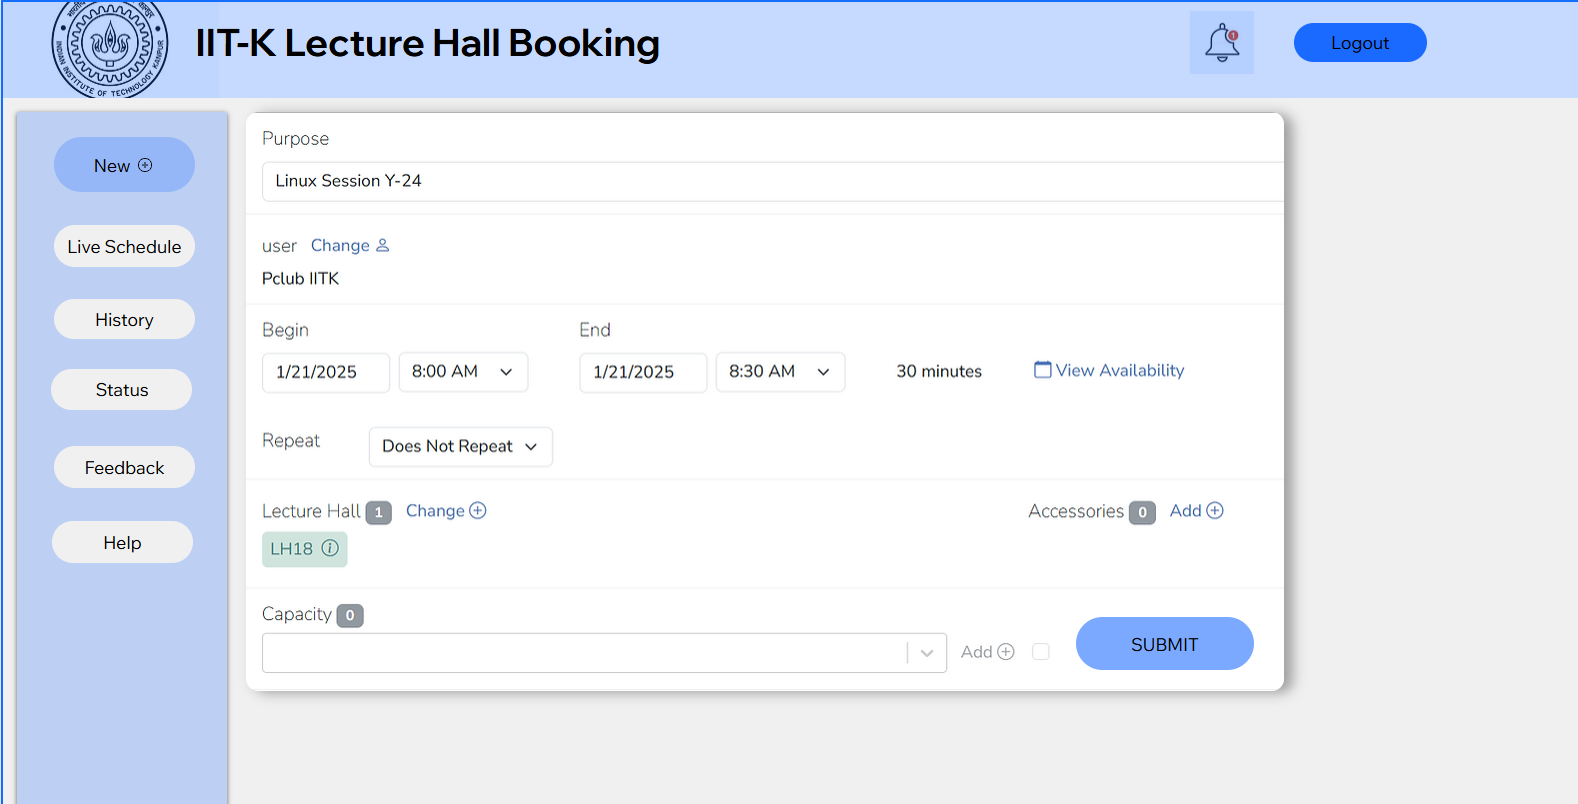
\includegraphics[width=1\textwidth]{form.png} 
    \caption{Request Submission Form}
    \label{form}
\end{figure}
    
    \begin{itemize}
        \item \textbf{Description:}
        \begin{itemize}
            \item After filling the form, the user can either:
            \begin{itemize} 
                \item Select a particular Lecture Hall, or
                \item Let the system select it automatically.
            \end{itemize}
            \item Real-time validation to ensure form completeness.
        \end{itemize}
        \item \textbf{Interaction:}
        \begin{itemize} 
            \item Text fields for: “Purpose”, “Capacity”
            \item Input fields for: “Date”, “Lecture Hall”, “Accessories”
            \item "Submit" button for finalizing the request.
            \item Interactive form fields with tooltips for assistance.
        \end{itemize}
    \end{itemize}
    \newpage
    \item \textbf{Admin Interface - History Tab}
    \begin{figure}[h!]
    \centering
    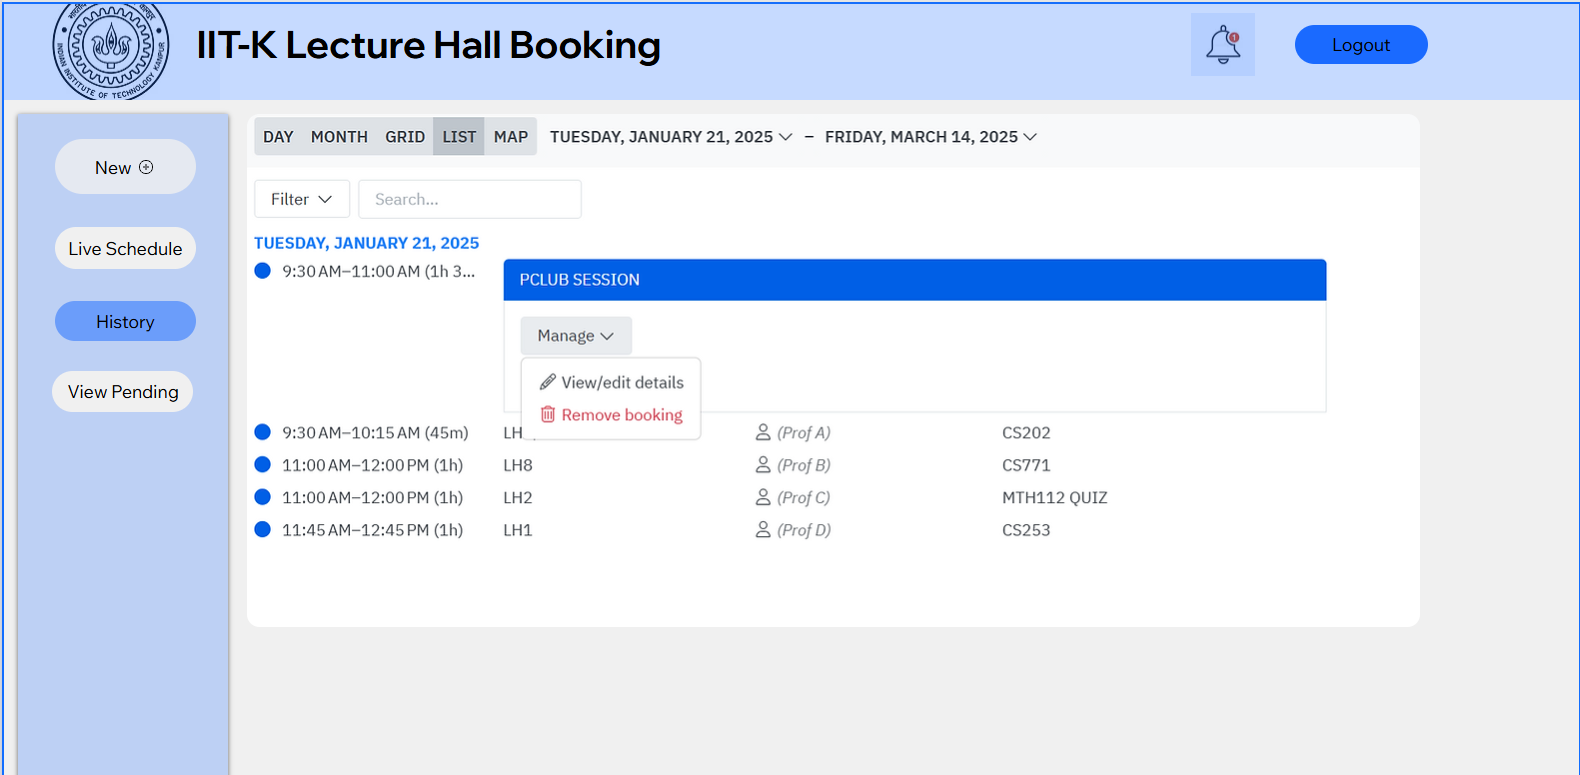
\includegraphics[width=1\textwidth]{his admin.png} 
    \caption{Admin Interface}
    \label{Fig 3.1.1 : Login Screen}
\end{figure}
    
    \begin{itemize} 
        \item \textbf{Description:}
        \begin{itemize} 
            \item This interface is only accessible by Admin.
            \item Authorities and Office Staff will access requests via a list view.
            \item Each request entry will display essential details, such as: Status, Timestamps and Remarks
            \item Actions like: “View/edit details”, “Remove bookings” will be available for each entry.
        \end{itemize}
        \item \textbf{Interaction:}
        \begin{itemize} 
            \item Buttons to execute approval/rejection actions. 
            \item A Search bar to search for bookings.
            \item Filters for date, month, Location
        \end{itemize}
    \end{itemize}
\end{enumerate}
% \subsubsection{Hardware Interfaces}
\subsubsection{Hardware Interfaces} 
The application will \textbf{primarily} be a \textbf{web application}, with the possibility of extending to a mobile application if time permits. Therefore, the hardware interfaces involved include:
\begin{itemize}
    \item \textbf{User Devices}
    \begin{itemize} 
        \item \textbf{Personal Computers (PCs):} Users will interact with the application through their PCs to access features such as: submitting requests, checking statuses and managing their accounts
        \item \textbf{Mobile Phones:} If a mobile application is developed, users will access similar features on their smartphones, ensuring convenience and mobility.
    \end{itemize}
    
    \item \textbf{Lecture Hall/Office Staff Devices}
    \begin{itemize} 
        \item \textbf{Staff PCs:} Office staff will use their PCs to:
            Verify user requests
            Manage approvals
            Perform administrative tasks related to the system
    \end{itemize}
    
    \item \textbf{Authority Devices}
    \begin{itemize} 
        \item \textbf{PCs:} Authorities will use their computers to review and process user requests submitted via the system
        \item \textbf{Mobile Phones:} Through the mobile application, authorities can also accept or reject requests on the go, ensuring flexibility and efficiency.
    \end{itemize}
\end{itemize}

\subsubsection{Software Interfaces}

\begin {itemize} 
    \item \textbf{Database Management System (DBMS)}
    The application will utilize a database to store and manage data efficiently. This includes:
        \begin{itemize} 
            \item \textbf{User Data:} Profiles, credentials, and role-specific information.
            \item \textbf{Request Records:} Details of user-submitted requests, their statuses, and timestamps.
            \item \textbf{Verification Logs:} Logs of actions taken by the office staff and authorities for tracking purposes.
        \end{itemize}
    A relational database (e.g., MySQL, PostgreSQL) will be used based on project requirements.
    
    \item \textbf{Mail Client for Automatic Email Generation}
    The application will connect to a mail client or SMTP service (e.g., Gmail SMTP, Microsoft Outlook, or SendGrid) to automate email communication.
        \begin{itemize} 
            \item \textbf{Verification Emails:} Automatically sent to authorities for request verification.
            \item \textbf{Notifications:} Updates to users about request status changes or approvals.
        \end{itemize}
    
    \item \textbf{Authentication Services}
    \begin{itemize} 
        \item Integration with institutional authentication systems for specific user roles, such as office staff and authorities.
    \end{itemize}
    
    \item \textbf{Web Server and API Services}
    \begin{itemize} 
        \item A web server will host the application and serve client requests.
        \item RESTful APIs will facilitate communication between the frontend, backend, and external systems like databases or mail clients.
    \end{itemize}
    
    \item \textbf{Frontend Framework}
    \begin{itemize} 
        \item The application will use Next.js, a React-based framework, for building the user interface.
    \end{itemize}
\end{itemize}

% \newpage
\subsection{Functional Requirements} \label{subsec:functional}

\subsubsection{User Authentication}
\begin{itemize} 
    \item The system shall allow users (club coordinators, professors, and LHC employees) to log in using unique credentials, which will be provided by the admin.
    \item No “Sign up” or “Register” option will be provided, and all credentials shall only be created by LHC Office Staff.
    \item The system must ensure secure authentication using HTTPS and hashed passwords.
\end{itemize}

\subsubsection{LH Booking}
\begin{itemize} 
    \item The system shall provide users with an interface to select a date, time, LH, and capacity for booking.
    \item The system shall automatically identify user role based on their unique id and provide them with special permission and options. For example. A club coordinator shall not be able to book a LH for a Course Quiz or Exam.
    \item The system shall enable users to select the type of activity for which the hall will be booked. These activity types, such as a Quiz, Placement Session, Club Workshop, etc., will be predefined within the system. This functionality will assist the LHC staff in preparing and managing the event appropriately
    \item The system shall allow users to select additional equipment such as projectors, microphones, and blackboards.
    \item The system should automatically validate the availability of the selected hall and equipment before confirming the booking.
    \item Once requested, the system shall automatically send authentication mail to all required authorities for approval. Each authority shall receive a unique link to approve or reject the booking.
    \item The action of approving and rejecting requests shall be done by clicking on the link.
    \item All pending requests shall be auto-rejected after a specified time frame.
    \item The user should be able to select and request multiple rooms at once.
    \item The system shall notify the user of the approval/rejection status via mail once all authorities respond.
\end{itemize}

\subsubsection{Timetable}
\begin{itemize} 
    \item The system shall display a timetable view on the home page (as previously shown in \ref{dashboard}) showing the schedule of LH for a given date.
    \item The timetable shall include details such as the time slot, the name of the booking user, and the purpose of the booking.
    \item This shall be visible to all visitors of the web-app.
\end{itemize}

\subsubsection{Automated Invoice Generation}
\begin{itemize} 
    \item Once the booking is confirmed by all the authorities, the system shall automatically generate an invoice for the booking, which will include details of hall usage, equipment charges, and any additional costs.
\end{itemize}

\subsubsection{Notifications}
\begin{itemize} 
    \item The system shall send email notifications to users upon successful booking, approval, or rejection.
    \item The system shall notify the admin in case of conflicts or errors during booking.
\end{itemize}

\subsubsection{Administrative Functions}
The system shall provide an admin interface for the LHC office staff to:
    \begin{itemize} 
        \item View all bookings and their statuses.
        \item Add, update, or delete bookings.
        \item Generate monthly and annual reports for usage statistics of equipment and LHs.
    \end{itemize}

\newpage
\subsection{Use Case Model} \label{subsec:use_case_model}

 \subsubsection{Use Case \#1: User Submits Request (U1)}
\textbf{Author} – Chaitanya, Rahul \\\\
\textbf{Purpose} - To allow users to submit a request through the web or mobile application. The request will be stored in the database and sent to authorities for verification. \\\\
\textbf{Requirements Traceability} – 
\begin{itemize} 
    \item R1: The user must be able to log in securely.
    \item R2: The system must allow the user to submit a request form.
    \item R3: The request must be stored in the database and trigger email notification to authorities.
\end{itemize}
\textbf{Priority} - High – This is a core function of the application. \\\\
\textbf{Preconditions} - 
\begin{itemize} 
    \item The user must be logged into the system.
    \item The request form must be valid and complete.
\end{itemize}
\textbf{Post conditions} - 
\begin{itemize} 
    \item The request is stored in the database.
    \item An email notification is sent to the appropriate authorities.
    \item The user is notified of successful submission.
\end{itemize}
\textbf{Actors} – 
\begin{itemize} 
    \item Primary Actor: User (Club-coordinator/Professor/LHC staff)
    \item Supporting Actor: Database, Mail Client
\end{itemize}
\textbf{Exceptions} - 
\begin{itemize} 
    \item Database connection failure while saving the request.
    \item Email notification fails due to SMTP service issues.
    \item Validation errors in the request form.
\end{itemize}
\textbf{Includes} - 
\begin{itemize} 
    \item U3: Validate User Login.
    \item U8: Trigger Email Notification.
\end{itemize}
\textbf{Notes/Issues} - 
\begin{itemize} 
    \item Need to ensure the database is available and functional at all times.
    \item SMTP service configuration must be robust and tested to handle high traffic.
\end{itemize}
\begin{figure}[h!]
    \centering
    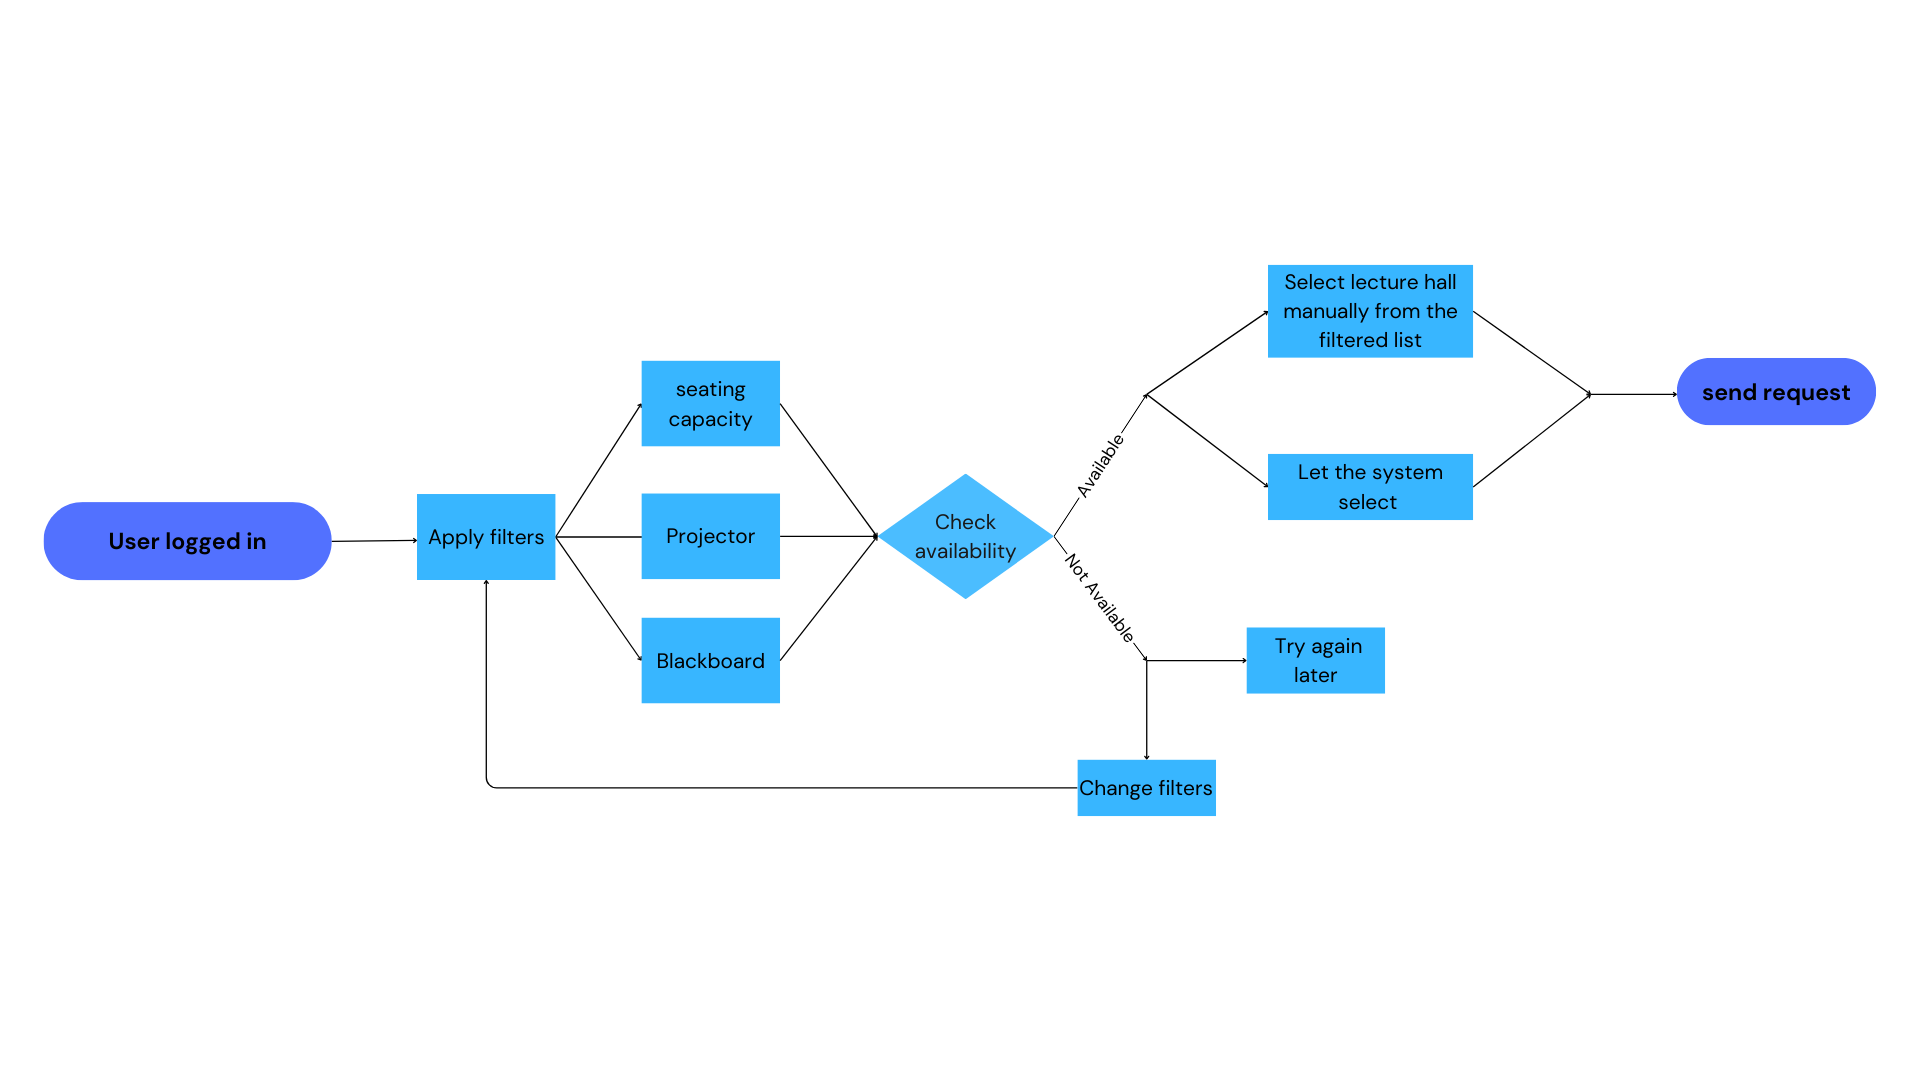
\includegraphics[width=1\textwidth]{U1.png} 
    \caption{Use Case 1}
    \label{Figure 3: Use Case 1}
\end{figure}
\newpage
 \subsubsection{Use Case \#2: Authority Verifies Request (U2)}
\textbf{Author} – Bhavya, Divyesh \\\\
\textbf{Purpose} - To allow authorities to review and approve or reject user-submitted requests. \\\\
\textbf{Requirements Traceability} – 
\begin{itemize} 
    \item R4: Authorities must receive a notification for each new request.
    \item R5: The system must display all relevant details of the request for verification.
    \item R6: The approval or rejection decision must be recorded in the database.
\end{itemize}
\textbf{Priority} - High – Ensures smooth processing of user requests. \\\\
\textbf{Preconditions} - 
\begin{itemize} 
    \item The request must exist in the system.
    \item The authority must be logged in securely.
\end{itemize}
\textbf{Post conditions} - 
\begin{itemize} 
    \item The approval/rejection decision is recorded in the database.
    \item The user is notified of the decision.
\end{itemize}
\textbf{Actors} – 
\begin{itemize} 
    \item Primary Actor: Authority
    \item Supporting Actor: Database, Mail Client
\end{itemize}
\textbf{Exceptions} - 
\begin{itemize} 
    \item Database errors during decision recording.
    \item Failure in notifying the user.
\end{itemize}
\textbf{Includes} - 
\begin{itemize} 
    \item U5: Notify User of Decision
\end{itemize}
\textbf{Notes/Issues} - 
\begin{itemize} 
    \item Ensure decision-making is logged for audit purposes.
    \item Handle cases where authorities fail to act on notifications.
\end{itemize}
\newpage
 \subsubsection{Use Case \#3: User Login (U3)}
\textbf{Author} – Atharv, Devansh \\\\
\textbf{Purpose} - To allow users to submit a request through the web or mobile application. The request will be stored in the database and sent to authorities for verification. \\\\
\textbf{Requirements Traceability} – 
\begin{itemize} 
    \item R7: Users must log in using valid credentials.
    \item R8: The system must differentiate roles (User, Office Staff, Authority) to grant appropriate access.
\end{itemize}
\textbf{Priority} - High – Ensures secure access and data protection. \\\\
\textbf{Preconditions} - 
\begin{itemize} 
    \item The user must have valid credentials (username and password).
    \item The database must store user credentials securely.
\end{itemize}
\textbf{Post conditions} - 
\begin{itemize} 
    \item The user is authenticated and granted access to role-specific features.
    \item Login activity is logged for security purposes.
\end{itemize}
\textbf{Actors} – 
\begin{itemize} 
    \item Primary Actor: User (Club-coordinator/Professor/LHC staff)
    \item Supporting Actor: Database
\end{itemize}
\textbf{Exceptions} - 
\begin{itemize} 
    \item Invalid credentials entered by the user.
    \item Database unavailability during login.
    \item Account locked due to multiple failed login attempts.
\end{itemize}
\textbf{Includes} - 
\begin{itemize} 
    \item U6: Validate Credentials
    \item U7: Log Activity
\end{itemize}
\textbf{Notes/Issues} - 
\begin{itemize} 
    \item Ensure encryption of passwords in the database.
    \item Implement a mechanism for password recovery.
\end{itemize}
\newpage
 \subsubsection{Use Case \#4: Generate Reports (U4)}
\textbf{Author} – Avantika, Aaradhya \\\\
\textbf{Purpose} - To generate and export reports on user requests, statuses, and actions for analysis and auditing. \\\\
\textbf{Requirements Traceability} – 
R9: The system must allow exporting data in various formats (e.g., CSV, PDF).
R10: Reports must be role-specific (e.g., user-specific, overall statistics).
\textbf{Priority} - Low – Not critical for initial deployment but valuable for audits and reviews. \\\\
\textbf{Preconditions} - 
\begin{itemize} 
    \item The data for reports must exist in the database.
    \item The user requesting the report must have appropriate access.
\end{itemize}
\textbf{Post conditions} - 
\begin{itemize} 
    \item A downloadable report is generated and made available to the user.
\end{itemize}
\textbf{Actors} – 
\begin{itemize} 
    \item Primary Actor: Office Staff, Authority
    \item Supporting Actor: Database
\end{itemize}
\textbf{Exceptions} - 
\begin{itemize} 
    \item Data query errors due to database inconsistencies.
    \item Large report sizes leading to processing delays.
\end{itemize}
\textbf{Includes} - 
\begin{itemize} 
    \item U9: Fetch Data for Report
\end{itemize}
\textbf{Notes/Issues} - 
\begin{itemize} 
    \item Ensure that sensitive information is excluded from reports based on roles.
    \item Optimize database queries to handle large datasets efficiently.
\end{itemize}
\newpage
 \subsubsection{Use Case \#5: User Feedback (U5)}
\textbf{Author} – Areen, Daksh \\\\
\textbf{Purpose} - To allow users to provide feedback on their experience with the application, report issues, or suggest improvements. The feedback will be stored in the database and accessible to the development team for review. \\\\
\textbf{Requirements Traceability} – 
\begin{itemize} 
    \item R11: The system must provide a feedback form accessible to all users.
    \item R12: Feedback must be stored in the database for analysis.
    \item R13: Feedback submissions must include optional user contact details for follow-up.
\end{itemize}
\textbf{Priority} - Medium – Improves the application through user insights but is not critical for initial deployment. \\\\
\textbf{Preconditions} - 
\begin{itemize} 
    \item The user must be logged into the application.
    \item The feedback form must be available and functional.
\end{itemize}
\textbf{Post conditions} - 
\begin{itemize} 
    \item The feedback is stored in the database.
    \item Optional notification is sent to the development team for high-priority feedback (e.g., bugs or critical issues).
\end{itemize}
\textbf{Actors} – 
\begin{itemize} 
    \item Primary Actor: User (Club-coordinator/Professor/LHC staff)
    \item Supporting Actor: Database
\end{itemize}
\textbf{Exceptions} - 
\begin{itemize} 
    \item Database errors while saving feedback.
    \item Failure to notify the development team about critical feedback.
\end{itemize}
\textbf{Includes} - 
\begin{itemize} 
    \item U11: Store Feedback in Database
    \item U12: Notify Development Team
\end{itemize}
\textbf{Notes/Issues} - 
\begin{itemize} 
    \item Ensure the feedback form is simple and intuitive.
    \item Implement spam detection mechanisms to prevent misuse.
    \item Classify feedback based on priority (e.g., bug reports, suggestions, general feedback).
\end{itemize}
\newpage
 \subsubsection{Use Case \#6: Notify User of Decision (U6)}
\textbf{Author} – Avantika, Aaradhya \\\\
\textbf{Purpose} - To inform the user about the approval or rejection of their submitted request via email or in-app notifications. \\\\
\textbf{Requirements Traceability} – 
\begin{itemize} 
    \item R14: The system must send notifications to users for all decisions made by authorities.
    \item R15: Notifications must include details of the decision and any relevant remarks.
\end{itemize}
\textbf{Priority} - High – Critical for ensuring users are informed about the status of their requests. \\\\
\textbf{Preconditions} - 
\begin{itemize} 
    \item A decision (approval or rejection) must be recorded in the database.
    \item The user must have provided valid contact information.
\end{itemize}
\textbf{Post conditions} - 
\begin{itemize} 
    \item The user is notified of the decision.
    \item The notification is logged for audit purposes.
\end{itemize}
\textbf{Actors} – 
\begin{itemize} 
    \item Primary Actor: Authority
    \item Supporting Actor: Database, Mail Client, Notification System
\end{itemize}
\textbf{Exceptions} - 
\begin{itemize} 
    \item Email notification fails due to SMTP service issues.
    \item In-app notification fails due to server errors.
\end{itemize}
\textbf{Includes} - 
\begin{itemize} 
    \item Log Notification in Database
    \item U14: Trigger Email/Notification
\end{itemize}
\textbf{Notes/Issues} - 
\begin{itemize} 
    \item Ensure email templates are clear and user-friendly.
    \item Provide fallback mechanisms for failed notifications, such as retries or alternative contact methods.
    \item Implement notification tracking to verify successful delivery.
\end{itemize}
\begin{figure}[h!]
    \centering
    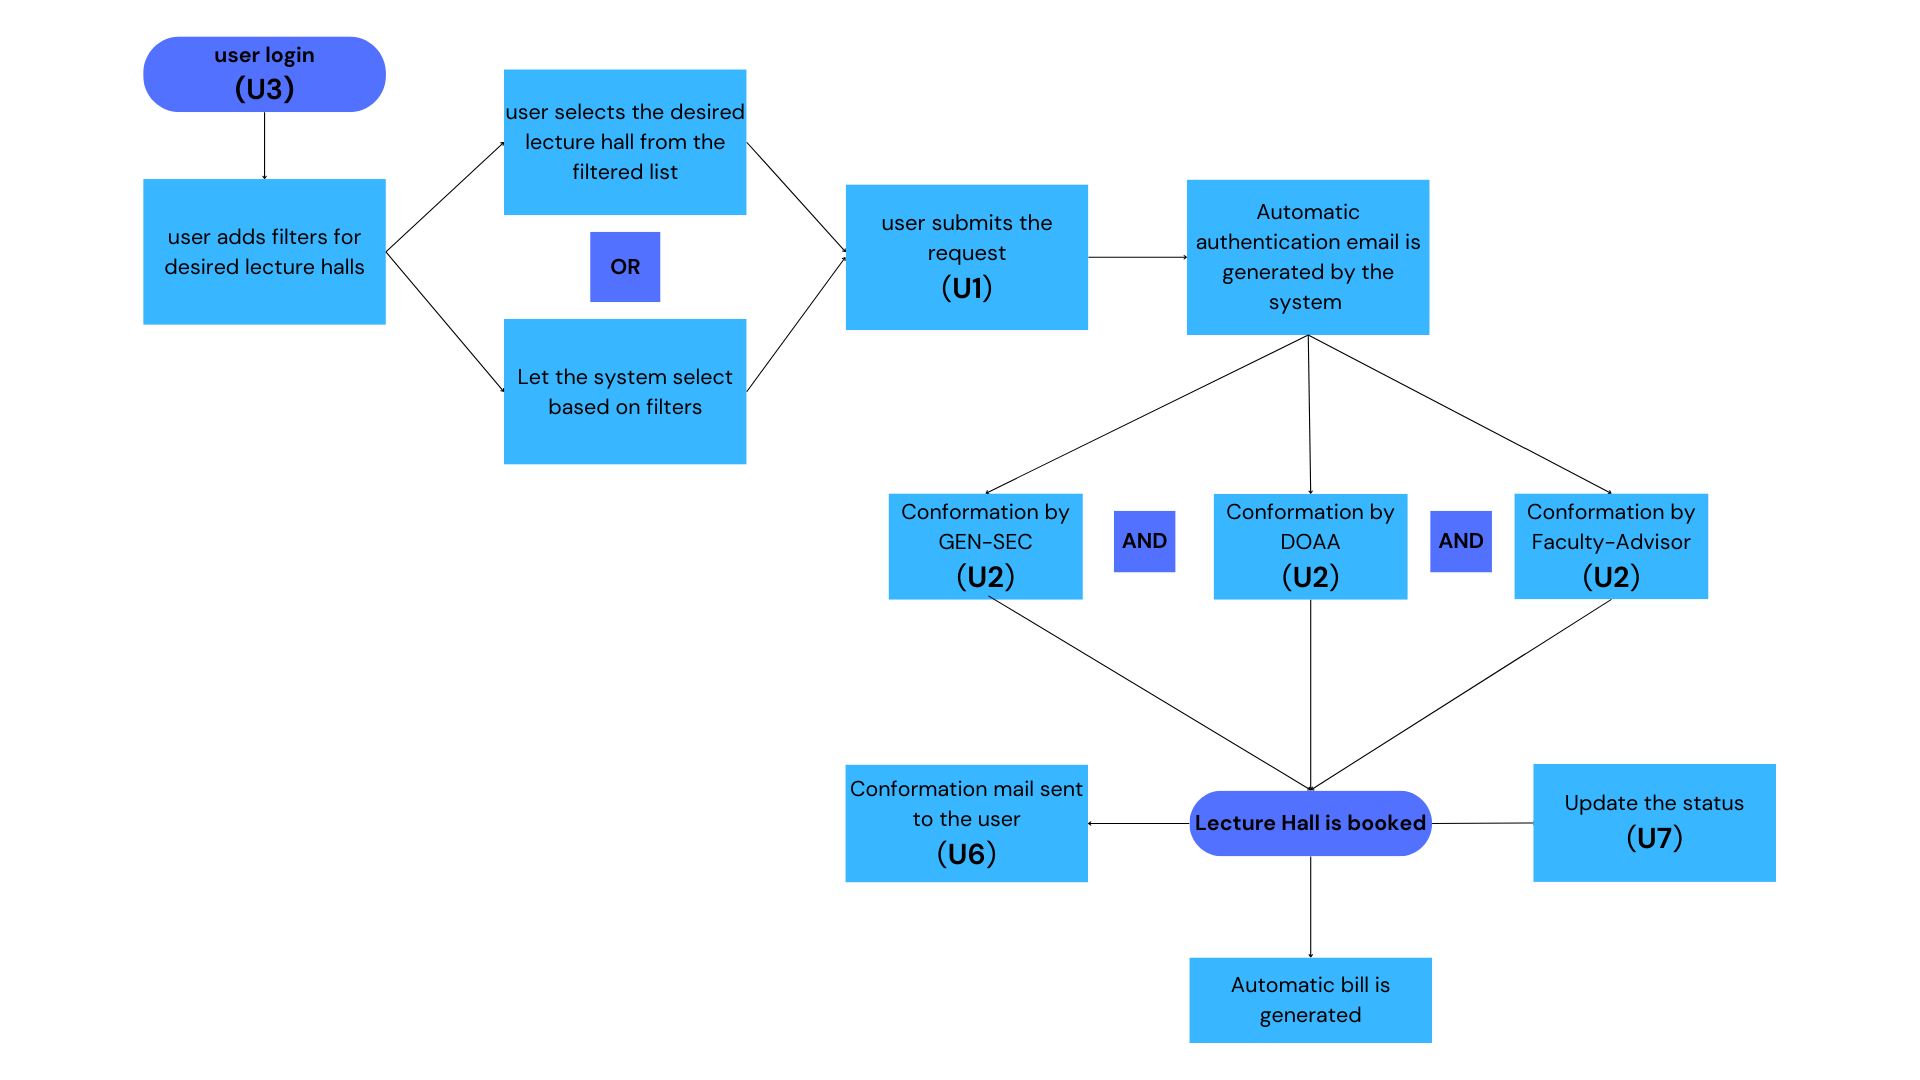
\includegraphics[width=1\textwidth]{final.png}
    \caption{Entire Use Case Diagram}
    \label{Figure 4: Entire Use Case Diagram}
\end{figure}

\clearpage

% Other Non-functional Requirements
\section{Other Non-functional Requirements} \label{sec:nonfunctional}
\subsection{Performance Requirements}\label{subsec:performance_reqs}
\begin{itemize}
    \item \textbf{System Response Time:} All UI interactions, such as clicking buttons, navigating menus, and searching for halls, must have a response time of \textbf{under 5 seconds} to maintain a smooth user experience.
    \item \textbf{Concurrent users:} The system should support \textbf{at least 20 concurrent users} without degradation in performance.
    \item \textbf{Real Time Updates:} 
The system should have real-time updates or near-real time of the booking confirmations in progress.
\vspace{-0.2em}
The booking confirmation can be confirmed or rejected by authority within \textbf{72 hours} of booking.
    \item \textbf{Scalability:} The system should scale seamlessly to support additional campuses or departments, increasing the number of users and lecture halls by \textbf{50\%} without requiring significant architectural changes.
    \item \textbf{Custom Reports:} On-demand custom reports, such as daily usage summaries or availability statistics, should generate and display within \textbf{5 seconds} for datasets containing up to \textbf{2,000 records}.
    \item \textbf{Throughput:} The system must handle at least \textbf{5 successful booking transactions per minute} during peak usage, ensuring a seamless experience for all users.

\end{itemize}

\subsection{Safety and Security Requirements} \label{subsec:security_reqs}
\begin{itemize}
    \item \textbf{User Education:} All users of the software must authenticate themselves using unique credentials (username and password) before accessing the system.
    \item \textbf{Session Management:} User sessions should automatically time out after 15 minutes of inactivity to prevent unauthorized access from unattended devices ensuring secure session handling to prevent session hijacking.
    \item \textbf{Audit Logs:} Maintain detailed logs of all critical actions, such as bookings, cancellations, or system changes, for auditing purposes. Logs must include timestamps, user identifiers, and the actions performed, and should be tamper-proof.
    \item \textbf{Safety Features:} Provide a confirmation step before finalizing any booking, cancellation, or deletion to prevent accidental actions. Include mechanisms to prevent double booking of lecture halls.
    \item \textbf{Security Warnings:} Notify administrators of any suspicious activities, such as multiple failed login attempts or attempts to access restricted areas of the system.
    \item \textbf{Access Control:}Sensitive administrative functions, such as editing or deleting bookings, should be restricted to authorized personnel.
    \item \textbf{Compliance with Institutional Policies:}  Align all safety and security measures with the institution’s IT policies and guidelines.
    \item \textbf{Privacy Requirements:} Personal data such as email addresses and booking history should only be accessible to the user and authorized administrators.

\end{itemize}

\subsection{Software Quality Attributes} \label{subsec:software_quality_reqs}

\subsubsection{Reliability}

\hspace{5mm}

\textbf{Requirement:} 

\begin{itemize}
    \item The lecture hall booking system shall ensure availability during working hours (8:00 AM to 10:00 PM) to ensure uninterrupted access for users. Any downtime for maintenance must be scheduled outside these hours and communicated to users at least 24 hours in advance.
\end{itemize}

\textbf{Plan to achieve:}
\begin{itemize}
\begin{itemize}
\begin{itemize}
    \item Implement automated monitoring and alert systems to detect and resolve issues proactively.
    \item Use redundant database backups to recover quickly in case of failures.
\end{itemize}

\end{itemize}

\end{itemize}

\subsubsection{Adaptability}

\hspace{5mm}

\textbf{Requirement:} 
\begin{itemize}
    \item The lecture hall booking system shall support the addition of new lecture halls, campuses, or user roles (e.g., event coordinators) without requiring significant code changes. The system should allow administrators to configure these settings via a web-based dashboard.
\end{itemize}

\textbf{Plan to achieve:}
\begin{itemize}

\begin{itemize}

\begin{itemize}
    \item Use a modular design and database schema that supports dynamic addition of entities (e.g., lecture halls, campuses, user roles).
    \item Implement a role-based access control (RBAC) mechanism to handle new roles easily.
\end{itemize}

\end{itemize}
\end{itemize}


\newpage

% Appendix
\appendix
\renewcommand{\appendixname}{Appendix}
\renewcommand{\thesection}{}
\section{Appendix A: Data Dictionary}
% \centering
% \resizebox{\textwidth}{!}{%
% \begin{tabular}{|l|p{5cm}|l|p{4cm}|p{4cm}|}
\hspace{-1cm}
\begin{longtable}{|>{\RaggedRight\arraybackslash}p{3.3cm}|p{2cm}|>{\RaggedRight\arraybackslash}p{5.5cm}|p{4cm}|}
    \hline
    \textbf{Item} & \textbf{Type} & \textbf{Description} & \textbf{Operations} \\
    \hline
    \endfirsthead
    \hline
    \textbf{Item} & \textbf{Type} & \textbf{Description} & \textbf{Operations} \\
    \hline
    \endhead
    \hline
    \endfoot

    % Constants
    \multicolumn{4}{|c|}{\textbf{Constants}} \\
    \hline
    \texttt{MAX\_HALLS} & Integer & Maximum number of lecture halls available for booking &System will not allow booking beyond this limit \\
    \hline
    \texttt{MAX\_BK\_DUR} & Integer & Maximum duration allowed for booking a lecture hall (in hours) & Typically 2 hours; system rejects bookings beyond this duration \\
    \hline
    \texttt{SYSTEM\_TIMEZONE} & String & The timezone in which the booking system operates & "Asia/Kolkata" or as per local setting \\
    \hline
    \texttt{price} & Integer & Variables assigning prices to each LH and equipment&System will use this to generate invoice \\
    \hline
    

        \hline
   \texttt{AUTO\_REJ\_TIME} & integer & The time in hours after the booking will be auto rejected. & typically 50-48 hours \\
    \hline


    % State Variables
    \multicolumn{4}{|c|}{\textbf{State Variables}} \\
    \hline
    \texttt{booking\_status} & String & Current status of the booking (e.g., "Available", "Booked", "Pending") & Operations: Update status when booking is made or canceled \\
    \hline
    \texttt{user\_role} & string & Role or designation of each user, normal\_user , admin, club, sop, professor, etc.& 
    Users are give special permission and validated based on their role\\
    \hline
    \texttt{hall\_id} & Integer & Unique identifier for each lecture hall & Operations: Generated during system setup, used to track bookings \\
    \hline
    \texttt{booked\_by} & String & Name or ID of the user who has booked the lecture hall & Operations: Updated when a booking is made \\
    \hline
    \texttt{booking\_time} & DateTime & Date and time of booking & Operations: Set when a user initiates a booking \\
    \hline
    \texttt{booking\_end\_time} & DateTime & End time of the booking & Operations: Set based on the start time and maximum booking duration \\
    \hline

    \texttt{activity\_type} & string & Type of activity the user will be using the LH for (e.g., "exam", "placement" , "session", "workshop" ,"lecture") & Operations: User selects while filling the request form\\
    \hline
    

    % Inputs
    \multicolumn{4}{|c|}{\textbf{Inputs}} \\
    \hline
    \texttt{user\_id} & Integer & ID of the user who is making the booking request & Operations: Verified against system user database \\
    \hline
    \texttt{req\_hall\_id} & Integer & LH ID that the user wants to book & Operations: Checked for availability in Database. \\
    \hline
    \texttt{req\_start\_time} & DateTime & Requested start time for booking & Operations: Checked for availability against other bookings \\
    \hline
    \texttt{req\_end\_time} & DateTime & Requested end time for booking & Operations: Checked for availability against other bookings \\
    \hline

    % Outputs
    \multicolumn{4}{|c|}{\textbf{Outputs}} \\
    \hline
    \texttt{bk\_confirmation} & String & Confirmation message or booking reference ID & Operations: Sent to the user upon successful booking \\
    \hline
    \texttt{error\_message} & String & Error or failure message (e.g., "Hall unavailable", "Invalid time slot") & Operations: Displayed to user if booking fails \\
    \hline
    \texttt{booking\_history} & List & A list of past bookings for a specific user or hall & Operations: Displayed when a user or admin checks booking history \\
    \hline
    \texttt{invoice\_number} & integer & Total cost of booking include equipment charge & Operations: Displayed to user when downloading invoice \\
    \hline

    % Functional Requirements
    \multicolumn{4}{|c|}{\textbf{Functional Requirements}} \\
    \hline
    \texttt{User Authentication} & Function & Verify if the user is authorized to make a booking & Operations: System must validate the user ID and password \\
    \hline
    \texttt{Hall Availability Check} & Function & Ensure requested hall is available at the requested time & Operations: Check if no conflicting bookings exist for the requested time \\
    \hline
    \texttt{Booking Request Approval} & Function & Admin must approve the booking request before it becomes final & Operations: Admin reviews and confirms booking requests \\
    \hline
    \texttt{Booking Confirmation} & Function & System sends confirmation upon successful booking & Operations: Email or SMS notification to the user \\
    \hline
    \texttt{Booking Cancellation} & Function & Users or admin can cancel bookings & Operations: Update the booking status, free the hall \\
    \hline
    \texttt{Invoice generation} & Function & System automatically generates invoice & Operations: Includes the overall cost of the booking. \\
    \hline
\end{longtable}

\newpage
\section{Appendix B: Group Log}
% \textit{Details of meetings and group activities.}
Since the beginning of the project, our entire team has been very enthusiastic.
We have formed a Whatsapp group for effective communication among the team members.

\begin{table}[h!]
\centering
\begin{tabular}{|m{4cm}|m{10cm}|}
\hline
\textbf{Meeting minutes} & \textbf{Agenda} \\ \hline
8 Jan 7:00 to 8:10 pm & We discussed a lot of different ideas and thought of different options. \\ \hline
& We discussed different ideas with Prof Indranil Saha and finalized an automated Lecture hall booking portal. \\ \hline
17 Jan 9:00 to 9:50 pm& planned out the draft of the SRS, discussed other logistics and deadlines, and started the work with full enthusiasm. \\ \hline
17 - 19 Jan & Worked out the draft of the SRS. We aligned our ideas and made a proper flow for the work.  \\ \hline
22 Jan & We met with the TA. We discussed the issues faced by the team. \\ \hline
23 Jan 9:00 to 10:30 pm & We were done with most of the raw work and went through the work done other members to avoid errors.and we went through the complete SRS once and discussed about the issues spotted\\ \hline
24 Jan& Gave the final touch to the SRS for the submission. \\ \hline

\end{tabular}
% \caption{Meeting Minutes Table}
% \label{tab:meeting_minutes}
\end{table}

\end{document}
